\section{Zgradba in sistemski pregled}
Razvojna plošča temelji na mikrokrmilniku ESP32-C3, ki podpira komunikacijo prek Wi-Fi-ja in BLE-ja. Glavne funkcionalnosti so prikazane na blokovni shemi (Slika~\ref{fig:blok_shema}).
Napajanje in komunikacija z računalnikom potekata prek USB-C priključka (MOLEX 216990-0001), skladnega z evropskimi standardi. Integrirani napetostni regulator skrbi za zanesljivo pretvorbo vhodnih 5 V na delovnih 3,3 V. Zasnova vključuje osnovne funkcionalne enote, kot so RGB LED, tipka in svetlobni senzor. Te enote omogočajo osnovne uporabniške interakcije in senzoriko.
Za stabilno delovanje skrbi več kondenzatorjev, ki blažijo napetostne spremembe in filtrirajo visokofrekvenčne motnje. Določeni upori delujejo kot pull-up elementi in zagotavljajo pravilna začetna logična stanja vhodov. Prehodni elementi (kot na primer stikala) so dodatno mehčani z RC kombinacijami, kar zmanjša pojav odbojev in zagotavlja zanesljiv zajem signala.
Plošča je odprtokodna in modularna. Omogoča enostavno nadgradnjo z zunanjimi komponentami prek dostopnih GPIO pinov. Zaradi podpore v Arduino okolju in široke skupnosti uporabnikov je GEMS Amethyst primerna tako za začetnike, kot za naprednejše razvojne projekte.

\begin{figure}[H]
    \centering
    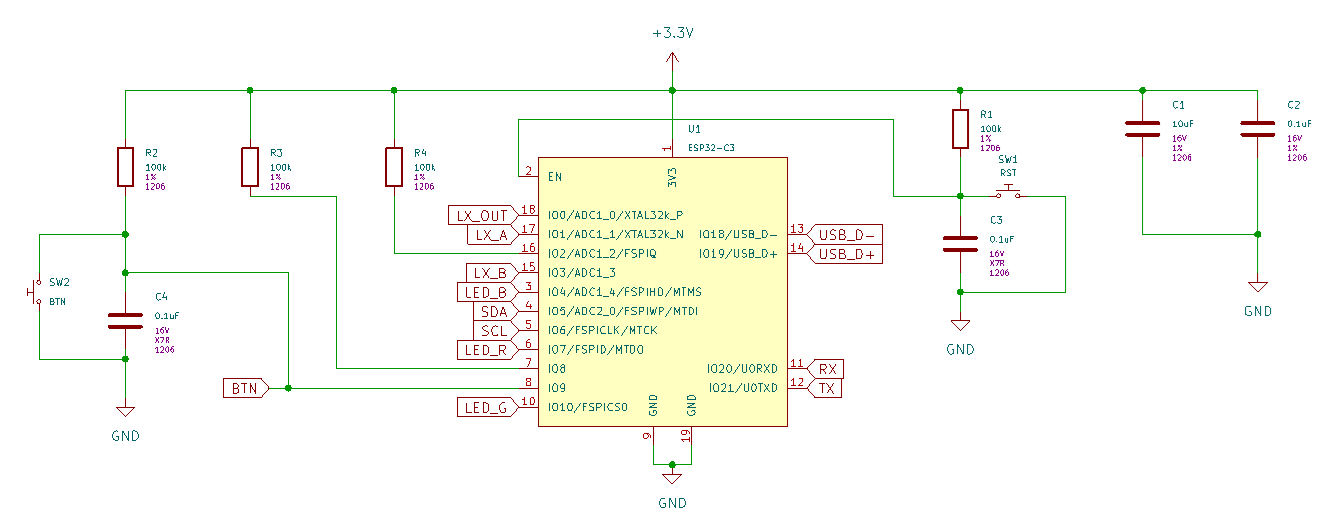
\includegraphics[width=1\textwidth]{Imgs/blok1.png}
    \caption{Blokovna shema razvojne plošče}
    \label{fig:blok_shema}
\end{figure}

\section{Sestavni elementi}
\begin{itemize}
    \item Mikrokrmilnik: ESP32-C3-WROOM-02 \\
    Povezava do podatkovnega lista: \url{https://eu.mouser.com/datasheet/2/891/Espressif_Systems_04082021_ESP32_C3_WROOM_02-2295851.pdf} \\
    Mikrokrmilnik predstavlja osrednji element razvojne plošče, saj upravlja delovanje vseh ostalih komponent in izvaja obdelavo podatkov. Gre za zmogljivo enoto s široko možnostjo uporabe – od osnovnega nadzora senzorjev do naprednejših aplikacij. Poleg klasičnih funkcij je podprta tudi brezžična komunikacija prek tehnologij Wi-Fi in BLE.

    \item USB-C priključek – Molex216990-001  \\
    Povezava do podatkovnega lista: \url{https://www.molex.com/content/dam/molex/molex-dot-com/products/automated/en-us/salesdrawingpdf/216/216990/2169900001_sd.pdf} \\
    Omogoča enostavno povezavo z računalnikom za napajanje in prenos podatkov.
    \begin{figure}[H]
        \centering
        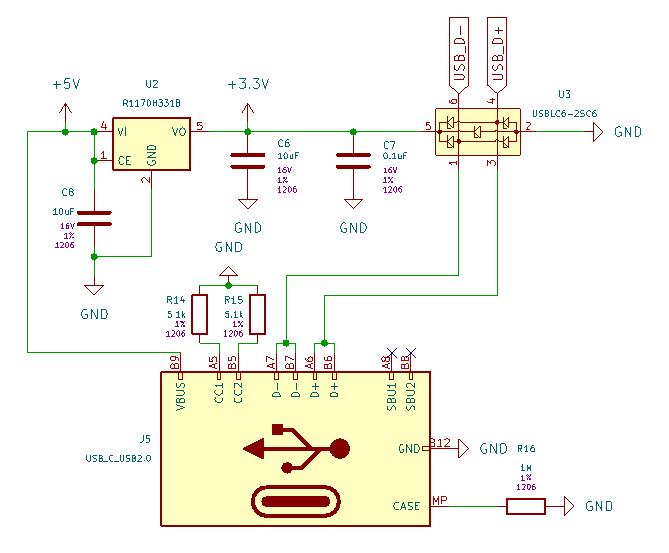
\includegraphics[width=0.8\linewidth]{Imgs/blok2.png}
        \caption{Blokovna shema USB-C priključka, ESD-ja in regulatorja napetosti}
        
    \end{figure}

    \item ESD(Electrostatic discharge) protection - USBLC6-2SC6 \\
    Povezava do podatkovnega lista: \url{https://eu.mouser.com/datasheet/2/389/usblc6_2-1852789.pdf} \\
    Gre za element, ki ščiti vezje pred škodljivimi vplivi elektrostatičnih razelektritev. Zaradi zelo nizke lastne kapacitivnosti ne vpliva na delovanje hitrih podatkovnih linij. Hkrati učinkovito omejuje tokovne sunke, ki bi lahko poškodovali občutljive komponente.

    \item LDO(Low dropout regulator) - R1170H331B-T1-FE \\
    Povezava do podatkovnega lista: \url{https://eu.mouser.com/datasheet/2/294/r1170_ea-3219814.pdf} \\
    Nizko-izgubni linearni regulator napetosti skrbi za pretvorbo vhodnih 5 V v stabilno delovno napetost 3,3 V. Izdelan je v CMOS tehnologiji, kar zagotavlja visoko energijsko učinkovitost, saj porabi energijo predvsem med preklopi stikalnih tranzistorjev.
    
    \item RGB LED - HV-5RGB60 \\
    Povezava do podatkovnega lista: \url{https://eu.mouser.com/datasheet/2/180/HV_5RGBXX_5mm_Full_Color_Series-1489147.pdf} \\
    Večbarvna LED dioda, z ločenimi rdečimi, zelenimi in modrimi elementi, omogoča generiranje različnih barv s pomočjo ustreznega krmiljenja PWM signalov. Standardni tok skozi diodo znaša 25 mA, maksimalni dovoljen impulz pa doseže do 100 mA za zelo kratek čas.
    
    \item Tipka - PTS645SM50SMTR92 LFS  \\
    Povezava do podatkovnega lista: \url{https://www.ckswitches.com/media/1471/pts645.pdf}  \\   
    Gre za SMD momentno stikalo, namenjeno ponastavitvi delovanja mikrokrmilnika med razvojem ali testiranjem programa. Zagotavlja mehansko zanesljivost do 100.000 pritiskov,  deluje do toka 50 mA pri napetosti 12 V.
    
    \item Senzor svetlobe - TEPT5700 \\
    Povezava do podatkovnega lista: \url{https://www.vishay.com/docs/81321/tept5700.pdf} \\    
    To je NPN fototranzistor, občutljiv na svetlobo v spektru vidne svetlobe. Z naraščanjem jakosti svetlobe se povečuje tok skozi senzor, kar omogoča zaznavo ambientne svetlobe.
    \begin{figure}[H]
        \centering
        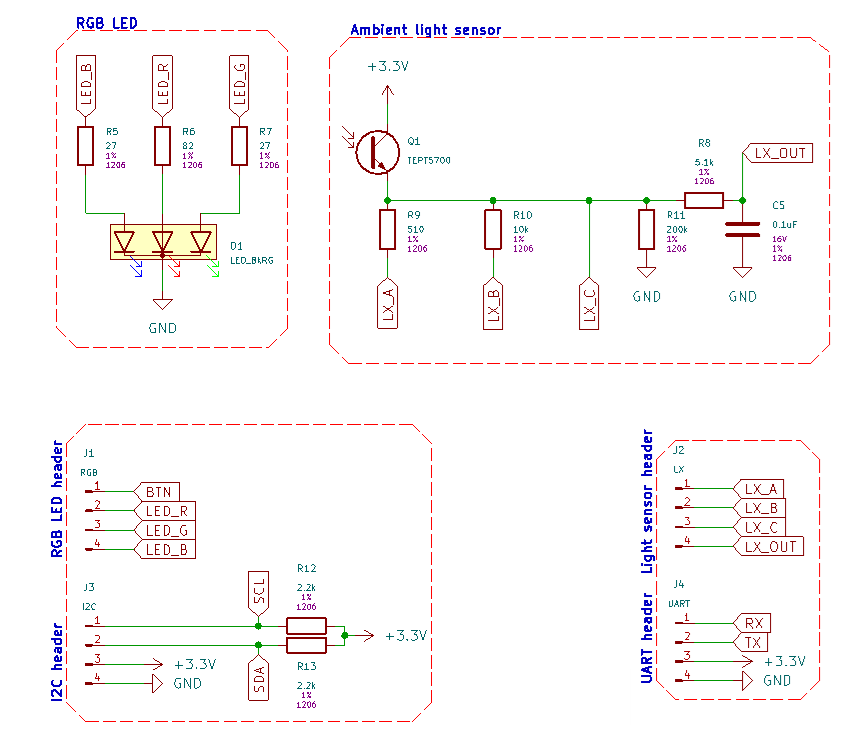
\includegraphics[width=0.9\linewidth]{Imgs/blok3.png}
        \caption{Blokovna shema ostalih modulov}
        \label{fig:enter-label}
    \end{figure}
\end{itemize}

\section{Razporeditev elementov}

\begin{figure}[H]
\centering
\begin{subfigure}{.4\textwidth}
  \centering
  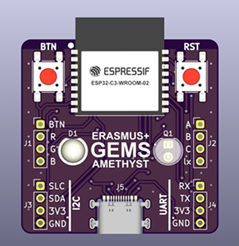
\includegraphics[width=.9\linewidth]{Imgs/board1.png}
\end{subfigure}
\begin{subfigure}{.4\textwidth}
  \centering
  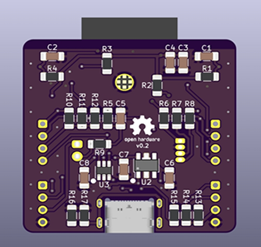
\includegraphics[width=.9\linewidth]{Imgs/board2.png}
\end{subfigure}
\caption{Razvojna plošča}
\end{figure}

\section{Tehnične specifikacije}
\begin{table}[H]
\centering
\caption{Tehnične specifikacije razvojne plošče GEMS Amethyst}
\begin{tabular}{|l|p{10cm}|}
\hline
\textbf{Parameter} & \textbf{Vrednost} \\
\hline
Mikrokrmilnik & ESP32-C3-WROOM-02 (RISC-V 32-bitni, 160 MHz, Wi-Fi + BLE 5.0) \\
\hline
Vhodna napetost (USB) & 5 V prek USB-C \\
\hline
Obratovalna napetost & 3.3 V (regulirana) \\
\hline
Maksimalni izhodni tok & 300 mA \\
\hline
Tipična poraba toka & $\sim$80 mA aktivno (Wi-Fi vklopljen), <10 µA v globokem spanju \\
\hline
Brezžični vmesniki & Wi-Fi 802.11 b/g/n (2.4 GHz), Bluetooth LE 5.0 \\
\hline
USB vmesnik & USB 2.0 Full-Speed (z ESD zaščito) \\
\hline
ESD zaščita & $\pm$15 kV (zrak), $\pm$8 kV (kontakt) \\
\hline
Senzor svetlobe & TEPT5700 – največja občutljivost pri $\sim$570 nm (vidna svetloba) \\
\hline
Podprti vmesniki & UART, SPI, I\textsuperscript{2}C, PWM, ADC (12-bitni), GPIO \\
\hline
Dimenzije plošče & 45mm x 40mm \\
\hline
Obratovalna temperatura & -40~$^\circ$C do +85~$^\circ$C \\
\hline
\end{tabular}
\label{tab:amethyst_spec_sl}
\end{table}



\section{Fizične povezave in izdelava}
Plošča uporablja dvoplastni PCB, ki vsebuje več plasti bakra. Te plasti omogočajo povezavo med različnimi elektronskimi komponentami na plošči. V našem primeru imamo bakrene plasti na obeh straneh plošče. Glavna funkcija bakrenih plasti je zagotavljanje poti za električne signale med različnimi komponentami na PCB-ju. Te poti so oblikovane kot sledilne poti, ki so izrezane iz bakrene plasti. Na zunanji plasti bakra se oblikujejo plastični odseki, ki so izolirani od zunanjih plasti ter med seboj s plastmi epoksidne smole. Proces izdelave PCB-ja se začne z načrtovanjem vezja v elektronskem CAD programu (KiCad), kjer se določijo postavitve komponent, sledi bakra in lokacije lukenj za montažo. Nato se izdela fotomaska, ki temelji na načrtovanem vezju in vsebuje informacije o sledi poti ter lokacijah lukenj za komponente. Substrat PCB-ja se pripravi z nanašanjem tankih plasti bakra (sledi poti) na obeh straneh. Sledi se ustvarijo s pomočjo fotomaske, ki ščiti bakreni sloj med izpostavljanjem izbranih delov bakra UV svetlobi za utrjevanje sledi. Nezaščiteni deli bakra se nato jedkajo, da se ustvarijo sledi za električne povezave. Po tem se izvrta luknje za montažo komponent. Na koncu sledi še namestitev komponent na PCB in pritrditev komponent z lotanjem. Pri oblikovanju PCB-ja je pomembno upoštevati širino in debelino sledilnih poti (traces) ter razporeditev bakrenih plasti, da se zagotovi ustrezna električna zmogljivost in zanesljivost vezja. Poleg tega se bakrene plasti uporabljajo tudi za izdelavo površinskih kontaktnih točk, ki omogočajo pritrditev in lotanje elektronskih komponent na PCB-ju.

Pri spajkanju elementov, kot so upori, pa je potrebna pazljivost.

\textbf{Navodilo za spajkanje:}
\begin{itemize}
    \item Najprej pripravimo razvojno ploščico in komponente, ki jih želimo lotati. 
    \item Potem namažemo ploščico s flux-om. 
    \item Nastavimo spajkalnik na približno 350 °C. 
    \item Nanesemo majhno količino spajke na eni strani kontakta, drugo stran lotamo potem. 
    \item Položimo komponente na kontakte ter s spajkalnikom zgrejemo spajke in tako ustvarimo povezave. 
    \item Ko smo končali z lotanjem vseh uporov na eni strani, potem zalotamo še drugo stran. 
    \item Na koncu preverimo vse lotane povezave in se prepričamo, da ni hladnih spojev ali kratkih stikov.
\end{itemize}

\textbf{Primer spremembe povezave:} Odklop LED in priklop zunanje LED prek pina LED\_R z uporom.